The Table \ref{tab:sdnn_table_noBase} presents the average heartbeat variance by each participant on each scenes and they are plotted in the Figures \ref{fig:barplot_ecg_sdnn_4_scene_blind} to \ref{fig:barplot_ecg_sdnn_4_scene}.


\begin{table}[!htb]
\centering
\caption{Average SDNN by the participants during the each round and method [ms].}
\label{tab:sdnn_table_noBase}
\begin{tabular}{lllrrrrr}
\toprule
    &       &        &   Audio &  \begin{tabular}[c]{@{}l@{}}Haptic\\ Belt\end{tabular} &  \begin{tabular}[c]{@{}l@{}}Virtual\\ Cane\end{tabular} &  Mixture \\
Part. & \begin{tabular}[c]{@{}l@{}}Visual\\ Condition\end{tabular} & Round &         &                                                        &                                                         &          \\
\midrule
001C & Blind & First & 107.061 &                                                124.737 &                                                 163.968 &  129.054 \\
    &       & Return & 130.885 &                                                131.590 &                                                 157.589 &  124.786 \\
002C & Blind & First &  98.863 &                                                 81.140 &                                                  33.977 &   79.289 \\
    &       & Return &  49.627 &                                                 42.815 &                                                 114.057 &  107.545 \\
003C & Blind & First &  38.325 &                                                 35.101 &                                                  42.392 &   43.692 \\
    &       & Return &  41.196 &                                                 44.256 &                                                  42.602 &   46.145 \\
004C & Blind & First &  86.827 &                                                 62.560 &                                                  85.900 &   70.472 \\
    &       & Return &  74.895 &                                                 70.017 &                                                  66.089 &  104.040 \\
001 & Sight & First &  82.185 &                                                134.530 &                                                 134.773 &  225.408 \\
    &       & Return &  69.479 &                                                318.747 &                                                 116.003 &  136.507 \\
003 & Sight & First &  79.600 &                                                 51.782 &                                                  68.676 &   60.842 \\
    &       & Return &  45.709 &                                                 40.927 &                                                  66.323 &   47.823 \\
004 & Sight & First & 121.130 &                                                154.718 &                                                 128.477 &  125.947 \\
    &       & Return & 100.366 &                                                122.563 &                                                 140.115 &  119.260 \\
005 & Sight & First &  87.686 &                                                120.522 &                                                  88.591 &  102.796 \\
    &       & Return &  93.207 &                                                122.839 &                                                 141.305 &   96.035 \\
\bottomrule
\end{tabular}
\end{table}



The Figures \ref{fig:barplot_ecg_sdnn_4_scene_blind} and \ref{fig:barplot_ecg_sdnn_4_scene_sight} do not show a pattern. Some methods caused a decrease while other caused an increase on the SDNN. The Figure \ref{fig:barplot_ecg_sdnn_4_scene} that in all methods the SDNN of the sight users were higher than the blind users. That means that the sight users had a lower mental workload than the blind users.

\begin{figure}[!htb]
    \centering
    \begin{minipage}{\textwidth}
        \centering
        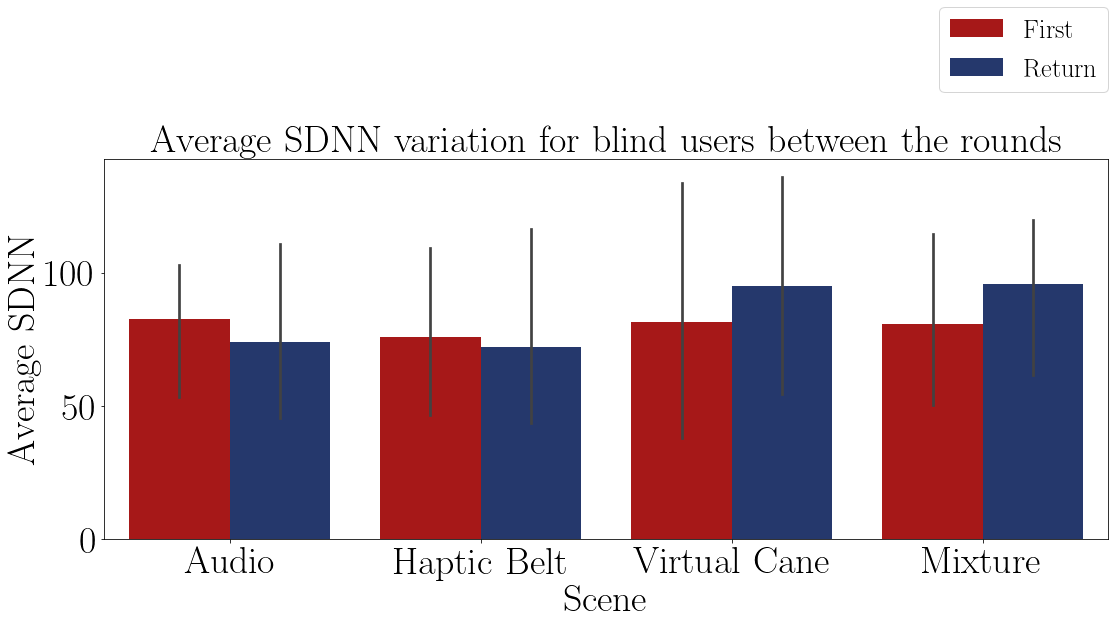
\includegraphics[width = 0.8\linewidth]{Resultados/ECG/Figuras/png/barplot_ecg_sdnn_4_scene_blind.png}
        \caption{Barplot of the average SDNN of the blind participants on each method and round.}
        \label{fig:barplot_ecg_sdnn_4_scene_blind}
    \end{minipage}
    \begin{minipage}{\textwidth}
        \centering
        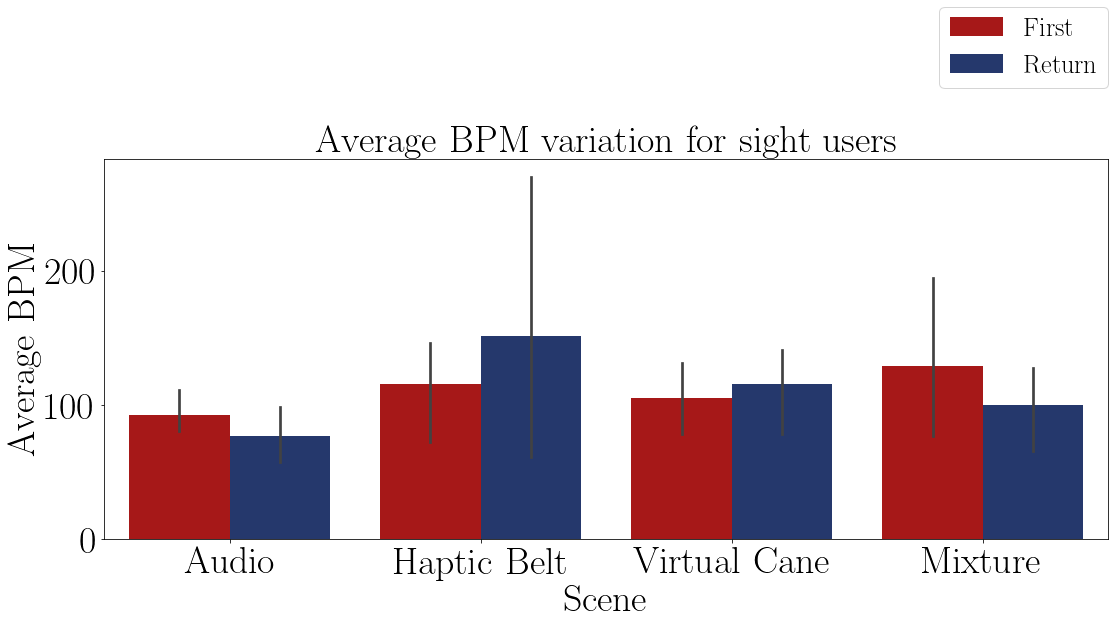
\includegraphics[width = 0.8\linewidth]{Resultados/ECG/Figuras/png/barplot_ecg_sdnn_4_scene_sight.png}
        \caption{Barplot of the average SDNN of the sight participants on each method and round.}
        \label{fig:barplot_ecg_sdnn_4_scene_sight}
    \end{minipage}
\end{figure}
\begin{figure}[!htb]
    \centering
    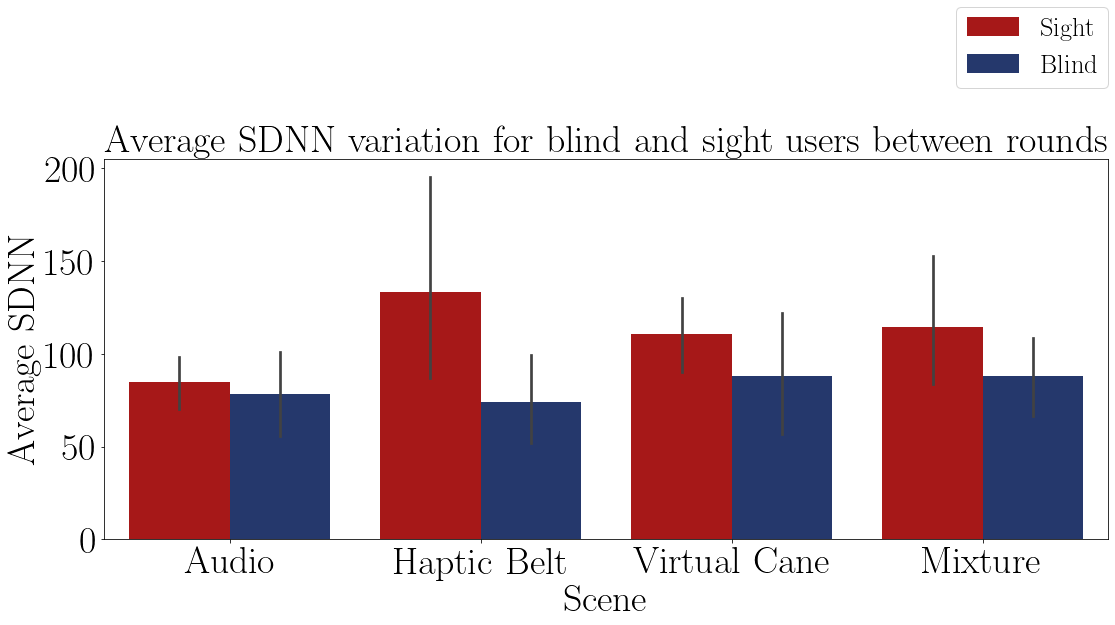
\includegraphics[width = 0.8\linewidth]{Resultados/ECG/Figuras/png/barplot_ecg_sdnn_4_scene.png}
    \caption{Barplot of the average SDNN of both participants on each method.}
    \label{fig:barplot_ecg_sdnn_4_scene}
\end{figure}

The Figure \ref{fig:boxplot_ecg_sdnn_4_scene} and \ref{fig:boxplot_ecg_sdnn_4_rounds} presents a box plot with the average SDNN of both groups by method and rounds in that order. These figures show the reaction of the sight user was a little different from the blind users. In all methods and rounds the SDNN from the sight users appear to be higher, hence with lower mental workload.

\begin{figure}[!htb]
    \centering
    \begin{minipage}{0.45\textwidth}
        \centering
        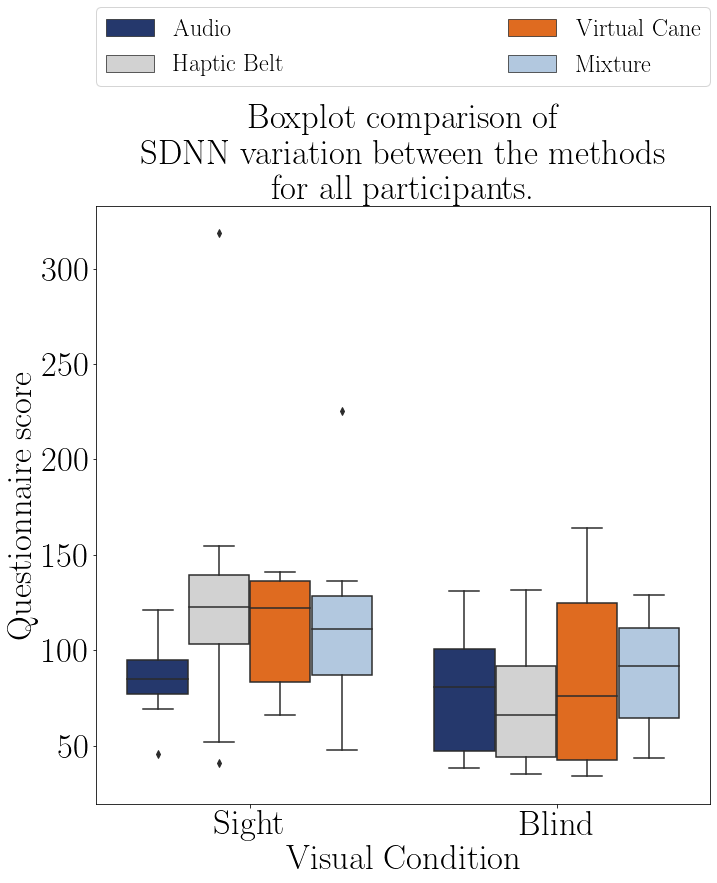
\includegraphics[width = 0.8\linewidth]{Resultados/ECG/Figuras/png/boxplot_ecg_sdnn_4_scene.png}
        \caption{Boxplot of the average SDNN of the participants grouped by method.}
        \label{fig:boxplot_ecg_sdnn_4_scene}
    \end{minipage}
    \begin{minipage}{0.45\textwidth}
        \centering
        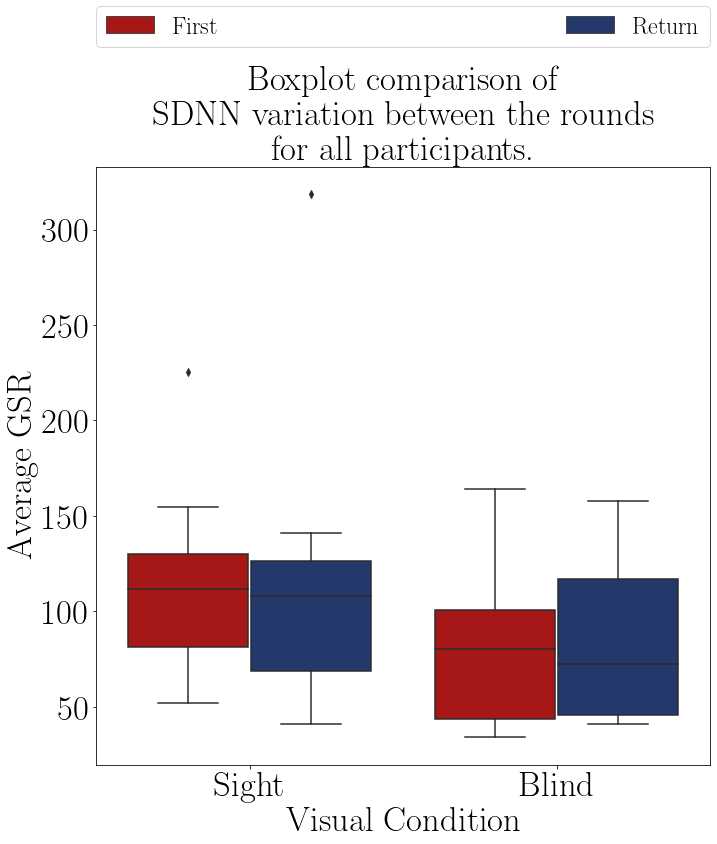
\includegraphics[width = 0.8\linewidth]{Resultados/ECG/Figuras/png/boxplot_ecg_sdnn_4_rounds.png}
        \caption{Boxplot of the average SDNN of the participants grouped by round.}
        \label{fig:boxplot_ecg_sdnn_4_rounds}
    \end{minipage}
\end{figure}
 
The Table \ref{tab:sdnn_average_group_noBase} shows the average heartbeat variance of both samples and is possible to notice how the average score by the sight users was higher in every method, reinforcing the Figures \ref{fig:barplot_ecg_sdnn_4_scene} to \ref{fig:boxplot_ecg_sdnn_4_rounds} conclusions.


\begin{table}[!htb]
\centering
\caption{ECG Average SDNN average in relation to the baseline grouped by participant and visual Condition.}
\label{tab:sdnn_average_group_noBase}
\begin{tabular}{lllrrrr}
\toprule
{} &  Audio & Haptic Belt & Virtual Cane & Mixture \\
Visual Condition &        &             &              &         \\
\midrule
Blind            &  78.46 &       74.03 &        88.32 &   88.13 \\
Sight            &  84.92 &      133.33 &       110.53 &  114.33 \\
\bottomrule
\end{tabular}
\end{table}



The Figures \ref{fig:qqplot_sdnn_two_way_sight} and \ref{fig:residplot_sdnn_two_way_sight} shows the distribution and variance of sighted participants of the Table \ref{tab:sdnn_table_noBase}. These Figures shows that the data are normally distributed and that the methods have a similar variance.
The Table \ref{tab:blocanova_sdnn_two_way_sight} shows the ANOVA test p-values of the average heartbeat variance of the "sight" sample between the guidance methods and they show that the methods had an effect on the score.


\begin{table}[!htb]
\centering
\caption{Anova p-value for the average SDNN on each method for blinded users.}
\label{tab:blocanova_sdnn_two_way_sight}
\begin{tabular}{lrrrrr}
\toprule
          Source & P-Value \\
\midrule
    \    Methods &   0.189 \\
     \    Rounds &   0.969 \\
\    Interaction &   0.455 \\
\bottomrule
\end{tabular}
\end{table}



\begin{figure}[!htb]
    \centering
    \begin{minipage}{0.45\textwidth}
        \centering
        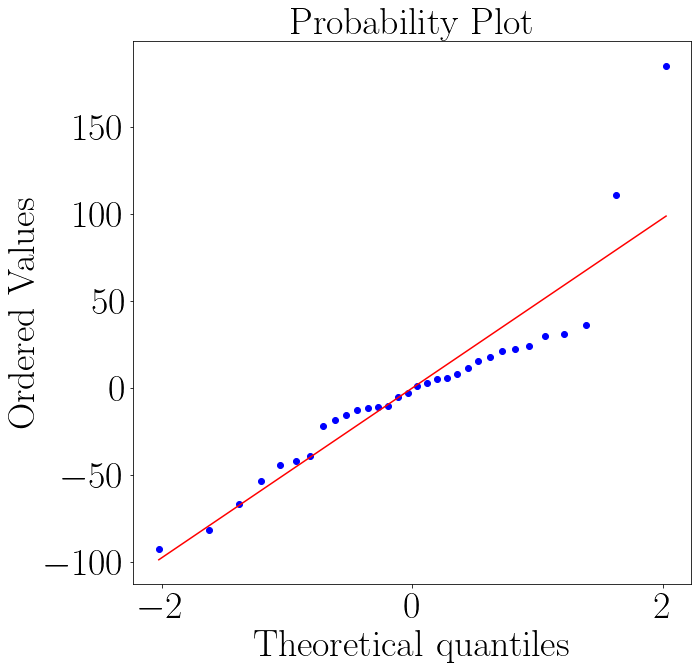
\includegraphics[width = 0.8\linewidth]{Resultados/ECG/Figuras/png/qqplot_sdnn_two_way_sight.png}
        \caption{QQ plot of the average SDNN of the sight participants on each method.}
        \label{fig:qqplot_sdnn_two_way_sight}
    \end{minipage}
    \begin{minipage}{0.45\textwidth}
        \centering
        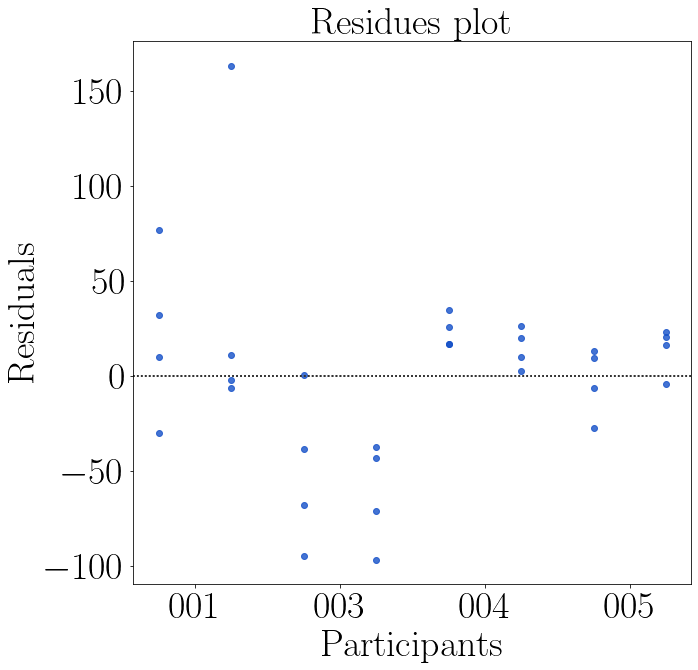
\includegraphics[width = 0.8\linewidth]{Resultados/ECG/Figuras/png/residplot_sdnn_two_way_sight.png}
        \caption{Residual plot of the average SDNN score the sight participants on each method.}
        \label{fig:residplot_sdnn_two_way_sight}
    \end{minipage}
\end{figure}


%
\begin{table}[!htb]
\centering
\caption{Cross validation p-value for the average SDNN on each method for blinded users.}
\label{tab:lsd_sdnn_two_way_sight}
\begin{tabular}{rclr}
\toprule
      \multicolumn{3}{c}{Method} &                          \multicolumn{2}{c}{Analysis} \\
\midrule
       Audio & $X$ & Haptic Belt &        $H_1 : \mu_{Audio} \ne \mu_{Haptic Belt}$ & ** \\
      Audio & $X$ & Virtual Cane &       $H_1 : \mu_{Audio} \ne \mu_{Virtual Cane}$ & ** \\
           Audio & $X$ & Mixture &            $H_1 : \mu_{Audio} \ne \mu_{Mixture}$ & ** \\
Haptic Belt & $X$ & Virtual Cane & $H_1 : \mu_{Haptic Belt} \ne \mu_{Virtual Cane}$ & ** \\
     Haptic Belt & $X$ & Mixture &      $H_1 : \mu_{Haptic Belt} \ne \mu_{Mixture}$ & ** \\
    Virtual Cane & $X$ & Mixture &         $H_0 : \mu_{Virtual Cane} = \mu_{Mixture}$ &  \\
\bottomrule
\end{tabular}
\end{table}


%
%The Table \ref{tab:lsd_sdnn_two_way_sight} presents the conclusion of a pairwise Fisher LSD test of the blind heart rate frequency variation between all the guidance methods and it shows that all methods had different effect on the heartrate, appart of the "Virtual Cane" and "Mixture", which presented similar SDNN.

According to the ANOVA test at Table \ref{tab:blocanova_sdnn_two_way_sight} there was no effect on the interbeat variance. So the methods did not influence the sighted user mental workload. The same conclusion was driven in the section \ref{subsubsec:results_ecg_1} in the SDNN part.

Also, the sight user had a higher SDNN, which means lower Mental Workload, a unexpected result based on the expectation and on the previous notes. 

\FloatBarrier